\documentclass{article}

\usepackage{graphicx}
\usepackage{tikz}
\usepackage{tikzsymbols}
\usetikzlibrary{calc,patterns,shapes.geometric}
\pagestyle{empty}
\usepackage[margin=0pt]{geometry}
\geometry{papersize={14in,12in}}

\def\centerarc[#1](#2)(#3:#4:#5){\draw[#1] ($(#2)+({#5*cos(#3)},{#5*sin(#3)})$) arc (#3:#4:#5);}

\begin{document}
	\begin{figure}
		\centering
		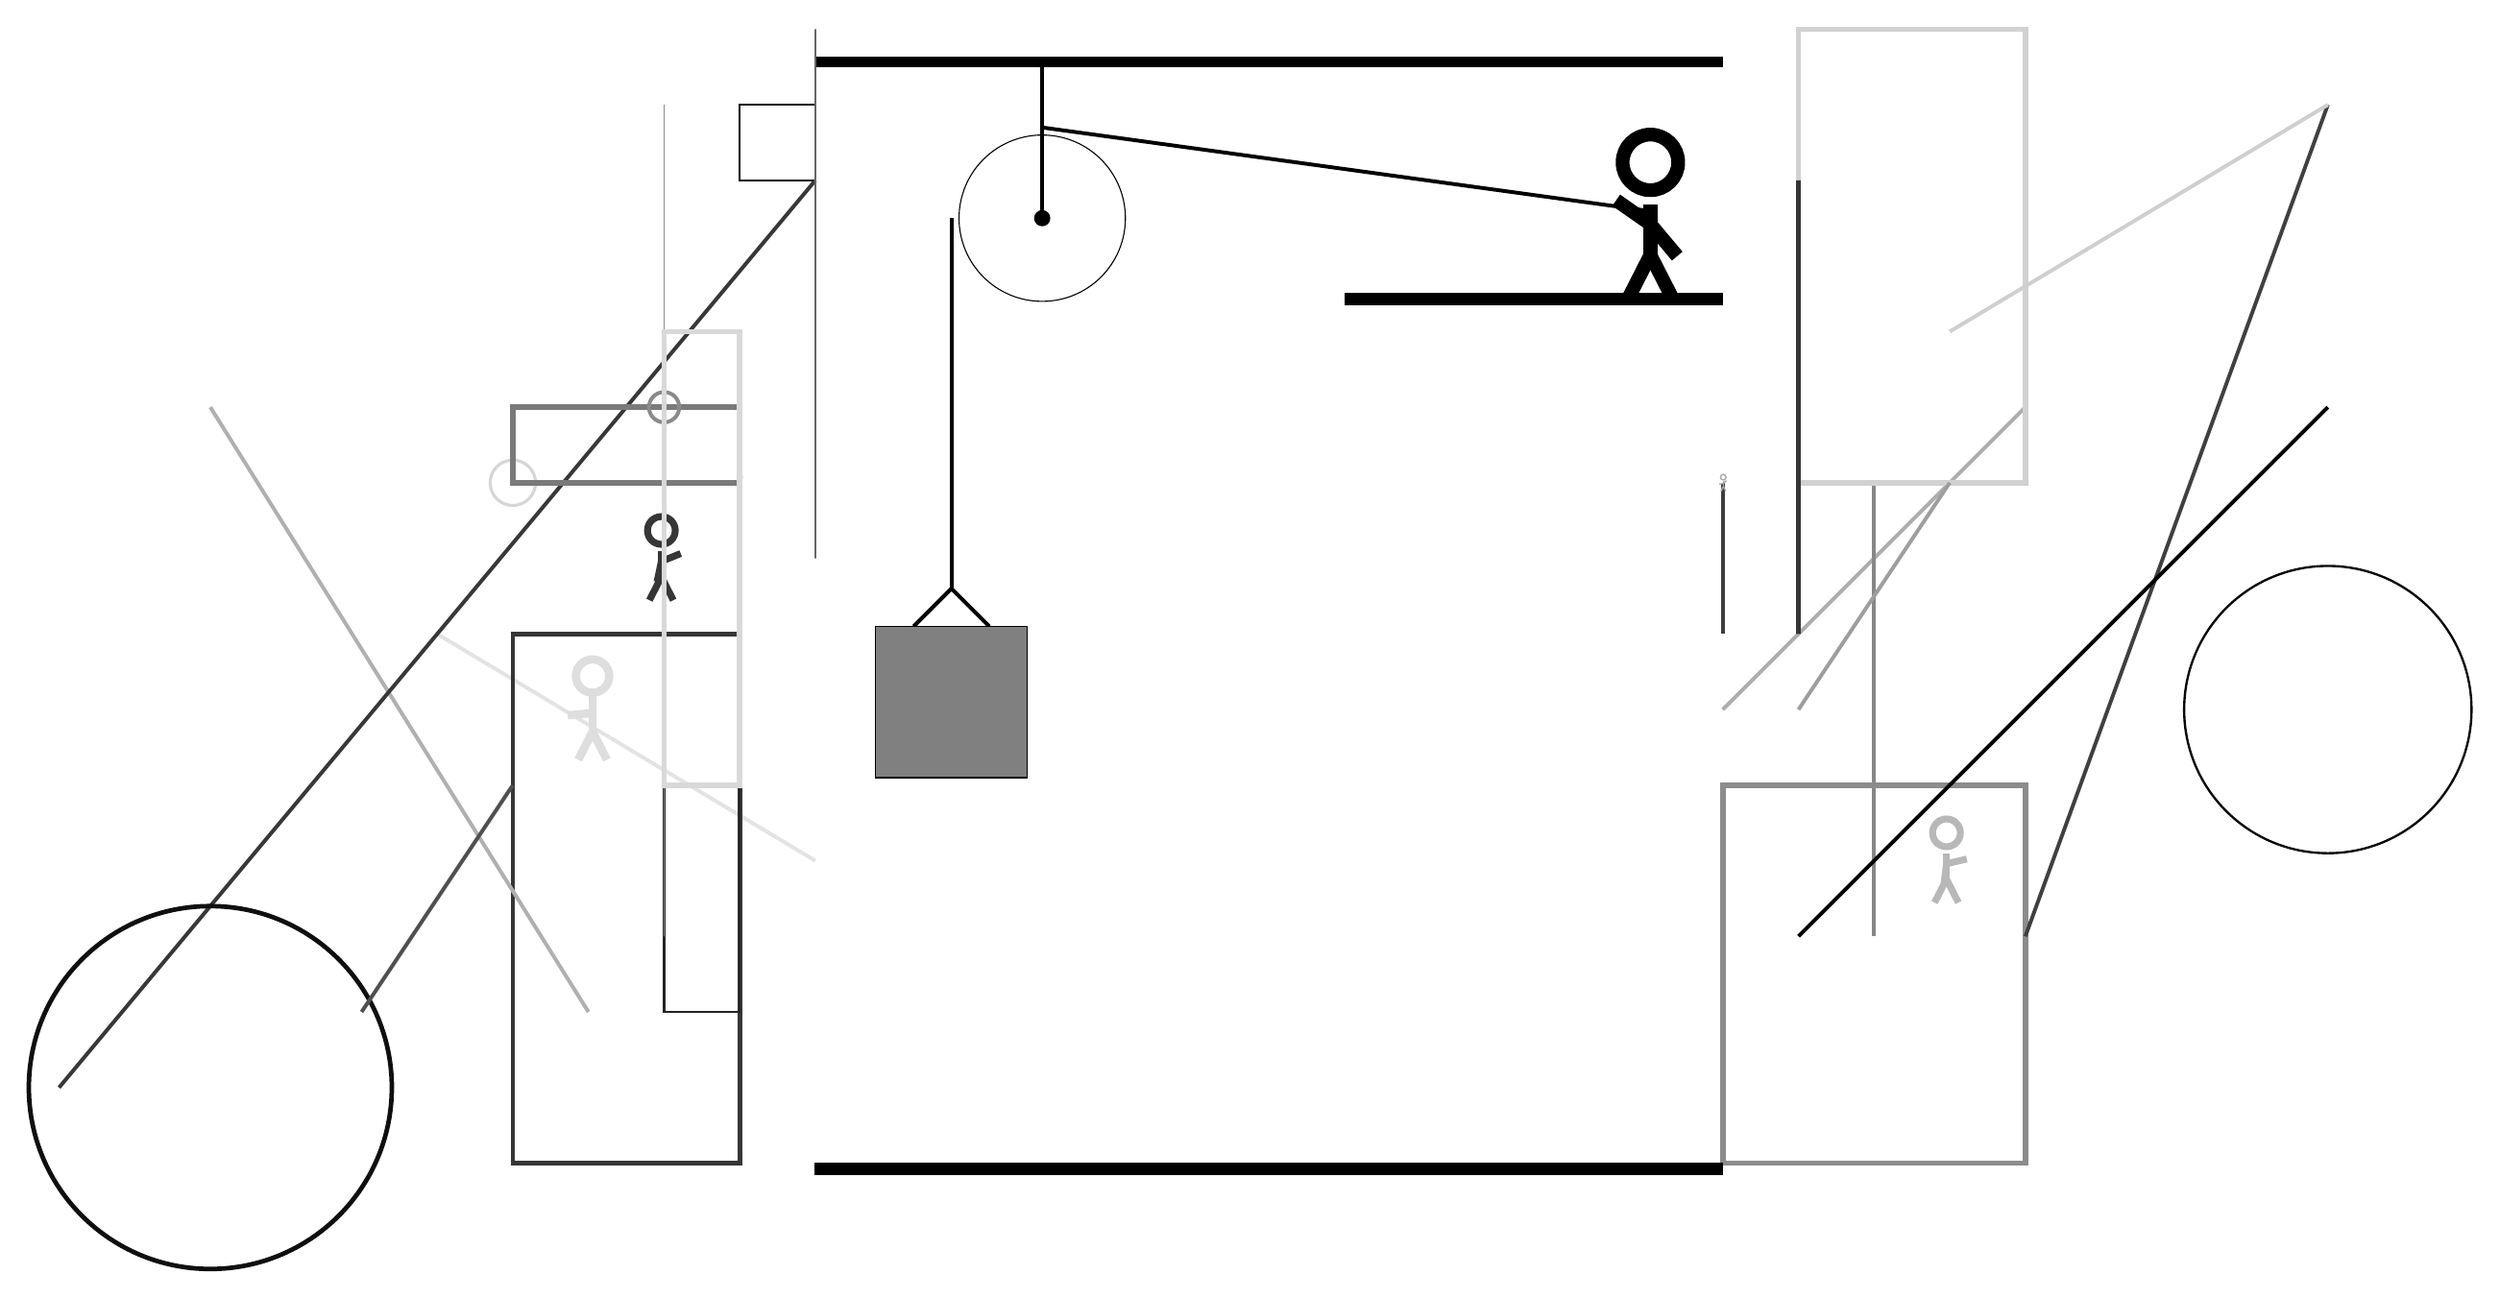
\begin{tikzpicture}
			%%%%% START %%%%%
			
			\draw[fill=black] (-2, 11.5) rectangle (10, 11.625);
			
			\draw (1, 9.5) circle (1.1);
			\draw[fill=black] (1, 9.5) circle (0.1);
			\draw[line width=0.5mm] (1, 11.5) -- (1, 9.5);
			
			\draw[line width=0.5mm, color=black!11](-2, 1) -- (-7, 4);
			
			\node[line width=0.7mm, color=black!79] at (-4, 5) {\Strichmaxerl[5][78][22]};
			\draw[line width=0.5mm, color=black!32](14, 7) -- (10, 3);
			\node[line width=0.3mm, color=black!28] at (13, 1) {\Strichmaxerl[5][83][13]};
			
			\draw[line width=0.5mm, color=black!47](12, 6) -- (12, 0);
			\draw [line width=0.3mm, color=black!97](18, 3) circle (1.9);
			\draw[line width=0.7mm, color=black!18] (11, 6) rectangle (14, 12);
			\draw[line width=0.7mm, color=black!45] (10, -3) rectangle (14, 2);
			\draw[line width=0.5mm, color=black!32](-3, 8) -- (-3, 6);
			
			\node[line width=0.3mm, color=black!13] at (-5, 3) {\Strichmaxerl[6][5][90]};
			\draw[line width=0.6mm, color=black!79] (11, 10) rectangle (11, 4);
			\draw[line width=0.5mm, color=black!75](14, 0) -- (18, 11);
			\draw[line width=0.6mm, color=black!79] (-3, -3) rectangle (-6, 4);
			
			\draw [line width=0.4mm, color=black!16](-6, 6) circle (0.3);
			\node[line width=0.7mm, color=black!13] at (-3, 6) {\Strichmaxerl[1][84][88]};
			\draw[line width=0.3mm, color=black!95] (-3, 10) rectangle (-2, 11);
			
			\draw[line width=0.3mm, color=black!86] (-3, -1) rectangle (-4, 2);
			\draw[line width=0.2mm, color=black!45] (-4, 11) rectangle (-4, 0);
			\draw[line width=0.5mm, color=black!38](11, 3) -- (13, 6);
			
			\draw[line width=0.5mm, color=black!31](-5, -1) -- (-10, 7);
			\draw[line width=0.5mm, color=black!78](-2, 10) -- (-12, -2);
			
			\draw[line width=0.5mm, color=black!19](13, 8) -- (18, 11);
			\draw [line width=0.6mm, color=black!94](-10, -2) circle (2.4);
			\draw[line width=0.7mm, color=black!52] (-3, 7) rectangle (-6, 6);
			\draw [line width=0.5mm, color=black!46](-4, 7) circle (0.2);
			
			\draw[line width=0.5mm, color=black!76](10, 6) -- (10, 4);
			\draw[line width=0.5mm, color=black!100](11, 0) -- (18, 7);
			\node[line width=0.5mm, color=black!33] at (10, 6) {\Strichmaxerl[1][11][41]};
			
			\draw[line width=0.5mm, color=black!69](-6, 2) -- (-8, -1);
			\draw[line width=0.2mm, color=black!60] (-2, 5) rectangle (-2, 12);
			\draw[line width=0.7mm, color=black!15] (-4, 8) rectangle (-3, 2);
			
			
			\draw[line width=0.5mm](-0.7, 4.1) --  (-0.2, 4.6) -- (0.3, 4.1);
			\draw[fill=black!50] (-1.2, 4.1) rectangle (0.8, 2.1);
			
			\draw[line width=0.5mm](-0.2, 9.5) -- (-0.2, 4.6);
			\centerarc[line width=0.5mm](1, 9.5)(90:180:1.2000000000000002)
			\draw[line width=0.5mm](1, 10.7) -- (9, 9.6);
			
			\node at (9, 9.5) {\Strichmaxerl[10][-35][-50]};
			\draw[fill=black] (5, 8.5) rectangle (10, 8.35);
			
			\draw[fill=black] (-2, -3) rectangle (10, -3.15);
			
			%%%%% END %%%%%
		\end{tikzpicture}
	\end{figure}	
\end{document}